\section{Conjunto de entrenamiento}
\subsection{Descripción}
Uno de los principales retos al trabajar con redes neuronales es la obtención de grandes conjuntos de entrenamiento que permitan mejores resultados, para el problema de reconocimiento de expresiones matemáticas existe una competencia llamada \textbf{Competition on Recognition of Online Handwritten Mathematical Expressions (CROHME)} que pone disponible de manera libre un conjunto de entrenamiento con mas de diez mil expresiones matemáticas escritas a mano provenientes de muchos usuarios voluntarios de distintos países mezclando los conjuntos de entrenamiento de 3 competencias CROHME. Se le pidió a los voluntarios copiar expresiones impresas de un \texttt{corpus} de expresiones. El corpus ha sido diseñado para cubrir la diversidad compuesta por las distintas tareas elegidas de un corpora matemático y de expresiones embebidas en páginas de wikipedia. Distintos dispositivos han sido utilizados (plumas digitales de distintas tecnologías, dispositivos de entrada como pizarrones blancos, tablets con pantalla sensible) de tal modo que distintas escalas y resoluciones son usadas %\cite{}.

\begin{figure}[h]
	\centering
	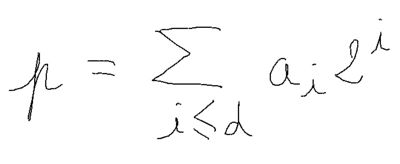
\includegraphics[width=0.4\textwidth]{capitulo5/dataset/crohme.jpg}
	\caption{Imagen de ejemplo del conjunto de datos de CROHME}
	\label{fig:crohme}
\end{figure}

A pesar de parecer un conjunto de datos prometedor para el desarrollo del presente trabajo terminal se deben considerar factores como el ruido que puede tener una imagen a partir de una fotografía tomada con un smartphone, por lo que se ha optado por utilizar una técnica denominada data aumentation que consiste en agregar ruido al conjunto de entrenamiento y otros procesos de análisis de imágenes como los mencionados en \ref{imAnalysis} permitiendo que el conjunto sea menos ideal y se puedan lograr mejores resultados 


